\documentclass{lab_class}

\usepackage{fancyhdr}
\pagestyle{fancy}
\rhead{П.\,Ю. Смирнов, 687 гр.}
\lhead{Лабораторная работа № 3.3.2, МФТИ, осень 2017}

\newcommand{\magm}{\mathfrak{M}}

\begin{document}

{\Large 3.3.2 -- Исследование вольт-амперной характеристики вакуумного диода.}

\paragraph{Цель работы.}
Определение удельного заряда электрона на основе закона <<трёх вторых>>.
В работе используются: вакуумный диод, микроамперметр, вольтметр, стабилизированные источники тока.

\paragraph{Теоретическая часть.}

\begin{wrapfigure}[12]{r}{4cm}
\centering
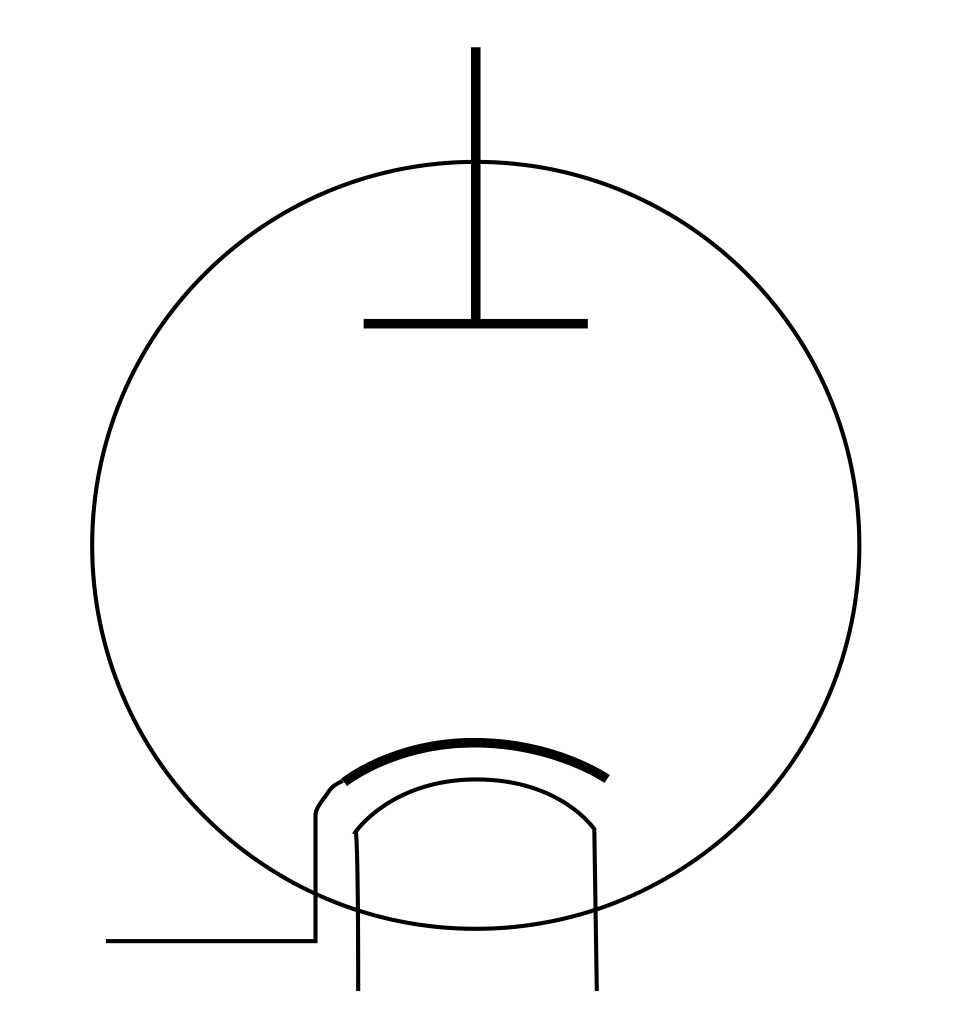
\includegraphics[width=3cm]{vacuum_diode.png}
\caption{Схема вакуумного диода}
\end{wrapfigure}

В основе работы вакуумного диода лежит явление термоэлектронной эмиссии, при которой электрон совершает работу выхода с поверхности твердого тела за счёт кинетической энергии теплового движения. Диод имеет простое устройство и состоит из двух частей -- катода и анода. На катод подается некоторый ток, называемый \emph{током накала}, за счёт которого он нагревается и эмитирует электроны. Между катодом и анодом подается постоянное напряжение, иными словами, создается постоянное электрическое поле, увлекающее к аноду эмитированные электроны -- возникает электрический ток. При постоянной температуре катода количество эмитируемых в единицу времени электронов постоянно, благодаря чему при некотором напряжении $U_{\text{нас}}$ возникает эффект насыщения. Более того, сила тока зависит от напряжения отнюдь не по линейному закону, поскольку поток электронов в пространстве между катодом и анодом создает некоторое дополнительное электрическое поле. Эта зависимость имеет степенной характер и называется \emph{законом <<трёх вторых>>}, или уравнением Шоттки:
\begin{equation}
	I = c V^{\frac{3}{2}}.
\end{equation}

Приведём её упрощенный вывод. Рассмотрим плоский диод (см. рисунок), направим ось $x$ перпендикулярно катоду в сторону анода. Тогда суть задачи сводится к решению одномерного уравнения Пуассона
\begin{equation}
	\dv[2]{\varphi}{x} = - \frac{\rho}{\varepsilon_0}.
\end{equation}
Плотность тока есть $j = \rho v$, скорость электронов определим из уравнения $\frac{m v^2}{2} = e \varphi$. При этом мы считаем, что потенциал катода нулевой, и пренебрегаем начальными тепловыми скоростями. Отсюда имеем дифференциальное уравнение
\begin{equation*}
	\dv[2]{\varphi}{x} = \sqrt{\frac{m}{2e\varphi}} j
\end{equation*}
с начальными условиями $\varphi(0) = 0$ и $\dv{\varphi}{x} (0) = 0$. Отсюда получаем
\begin{equation}
	I = \frac{4 \varepsilon_0 S}{9 d^2} \sqrt{\frac{2e}{m}} V^{\frac{3}{2}},
\end{equation}
где $d$ -- расстояние между электродами, а $S$ -- площадь катода. Мы видим, что исследование вольт-амперной характеристики вакуумного диода позволят нам определить удельный заряд электрона!

Оказывается, указанная степенная зависимость $I(V)$ не зависит от геометрии диода, а вот постоянный множитель ещё как. Решение похожей (малоинтересной) задачи для используемого в нашей лаборатории цилиндрического диода даёт следующий результат:
\begin{equation}
	I = \frac{8\sqrt{2}\pi\varepsilon_0 l}{9} \sqrt{\frac{e}{m}} \frac{1}{r_a \beta^2} V^{\frac{3}{2}},
\end{equation}
где $r_a$ -- радиус анода, $l$ -- расстояние между электродами, $\beta^2$ -- некая волшебная функция, возникающая при решении дифференциального уравнения. 

\end{document}